\documentclass{article}

% if you need to pass options to natbib, use, e.g.:
% \PassOptionsToPackage{numbers, compress}{natbib}
% before loading nips_2016
%
% to avoid loading the natbib package, add option nonatbib:
% \usepackage[nonatbib]{nips_2016}

%\usepackage{nips_2016}

% to compile a camera-ready version, add the [final] option, e.g.:
 \usepackage[final]{nips_2016}

\usepackage[utf8]{inputenc} % allow utf-8 input
\usepackage[T1]{fontenc}    % use 8-bit T1 fonts
\usepackage{hyperref}       % hyperlinks
\usepackage{url}            % simple URL typesetting
\usepackage{booktabs}       % professional-quality tables
\usepackage{amsfonts}       % blackboard math symbols
\usepackage{nicefrac}       % compact symbols for 1/2, etc.
\usepackage{microtype}      % microtypography
\usepackage{graphicx}

\title{Category Classification With Animal Image Data}

% The \author macro works with any number of authors. There are two
% commands used to separate the names and addresses of multiple
% authors: \And and \AND.
%
% Using \And between authors leaves it to LaTeX to determine where to
% break the lines. Using \AND forces a line break at that point. So,
% if LaTeX puts 3 of 4 authors names on the first line, and the last
% on the second line, try using \AND instead of \And before the third
% author name.

\author{
 Chudan Liu\\
 Department of Mathematics\\
 Harvey Mudd College\\
 Claremont, CA 91711 \\
 \texttt{iliu@g.hmc.edu} \\
 %% examples of more authors
  \And
  Xinyu Yang \\
  Department of Mathematics\\
  Harvey Mudd College \\
  Claremont, CA 91711 \\
  \texttt{xiyang@g.hmc.edu} \\
 %% \And
 %% Coauthor \\
 %% Affiliation \\
 %% Address \\
 %% \texttt{email} \\
}
\begin{document}
% \nipsfinalcopy is no longer used

\maketitle

\begin{abstract}
 
Image classification extracts the key features of images, analyzes the numerical properties of these features and classify the data into categories, which is one of the most important applications of deep learning to computer vision problems. Image classification, as a complex task for machines, has a wide range of application in real life, such as image retrieval, object detection, objection segmentation and object classification. This paper introduces multiple methods for object classification and evaluates the performance of each method through different experiments on species categories on animal image data. While image classification can be conducted through both supervised and unsupervised learning, we train an animal category predictor using logistic regression model, multilayer perceptrons neural network, support vector machines (SVM) with linear kernel and radial basis function kernel, which could be output and saved on disk. Then, we compare the performance of these predictors by computing their running time and accuracy through confusion matrix. With these models, we create an interactive animal classification that lays satisfying results in running time and validity scopes. 
\end{abstract}

\section{Introduction}
\paragraph{}
In this paper we are dealing with image classification problem, which is the job of assigning an input image one label from a fixed set of categories. This is one of the core problems in Computer Vision that, despite its simplicity, has a large variety of practical applications. Moreover many other seemingly distinct Computer Vision tasks (such as object detection, segmentation) can be reduced to image classification. Thus, image classification problem is the foundation of most of the image-based big data problem, including optical character recognition, edge detection, and object recognition.
\paragraph{}
For this project, we selected the Common Object in Context (COCO) dataset \url{http://mscoco.org/dataset}, a popular image recognition, segmentation, and captioning dataset to perform image classification. We chose this dataset because it has over 80,000 images with multiple objects and clear labels. We specifically look into the animal supercategory, which has 10 categories of different animals. The main task is to use these images and animal labels as input to train a classifier that can perform prediction.
\paragraph{}
Many useful algorithms for image classification have been developed throughout these years. For our project, we chose several different algorithms to train the classifiers and use various methods to evaluate these algorithms. We primarily focused on logistic regression model, multilayer perceptron neural network model, and support vector machine (linear and nonlinear kernel).
 
\paragraph{}
The major parts of this report are:
\begin{enumerate}
\item 
A summary of the algorithms we used in our project, with detail explanation and mathematical justification.
\item 
Extraction of the final dataset and training and testing data processing.
\item 
Performance analysis of each algorithms with an introduction to confusion matrix.
\item 
Experiment of how good the predictor actually works with several examples
\item 
Possible future works and applications
\end{enumerate}

\section{Learning Algorithms}
\paragraph{}
In our project, we used four algorithms to classify the data: Logistic Regression, muli-layer perceptron neural network (MLP), linear support vector machines and nonlinear support vector machines with radial basis function kernel. Below are details about the algorithm and parameters we used in this project. 
\subsection{Multinomial Logistic Regression}
\paragraph{}
Multinomial Logistic Regression is the first learning algorithm we used. Given a set of independent categorical variables, which are the pixels of animal images from our dataset in this case, we trained a logistic regression model to predict the probabilities of the different possible animals of the independent  categorical variables.
\paragraph{}
As most other statistical classification models, the foundation of the logistic regression model is to construct a linear predictor function that computes a score from a set of regression coefficients  that indicate the relative effect of variables on the $y$. In particular, \[
Score(k, X_i) = \beta_k \cdot X_i,
\]
where $k$ indicates the outcome  $k$, which is the category ID; $X_i$ is the vector of explanatory variables, which are all the pixels of an image describing observation $i$; $\beta_k$ is a vector of  regression coefficients corresponding to outcome k. For all $X_i$, the predicted outcome falls in the outcome with the highest score. If we denote the probability that the $X_i$ falls in category $k$ as \[ \pi_{ik} = P\{Y_i = k\},
\]
since the categories are mutually exclusive and exhaustive, $\pi_{ij}$ add up to one for each individual  image and we have \[ 
\sum_{k=1}^K \pi_{ik} = 1 \ \textbf{ for all }  i \]
\paragraph{}
To approach the multinomial data, we will nominate one of the outcome categories as a baseline cell, calculate the log-odds for all other categories relative to the baseline, and let the log-odds be a linear function of the predictor Score function. We assume the log-odds of each outcome category follow a linear model \[
\eta_{ik} = log \ \frac{ \pi_{ik} }{ \pi_{iK} } = \alpha_k + x_i'\beta_k
\]
where $\alpha_k$ is a constant and $\beta_k$ is a vector of regression coefficients for $k \in [1, K-1]$.
We can see that the logits are a quadratic function and therefore we will entertain the model \[
\eta_{ik} = \alpha_k + \beta_k \alpha_i + \gamma_k a_i^2 \]
where $a_i$ is the midpoint of the $i^{th}$ image and $k = 1, 2$ for the category ID among all of them respectively.


\subsection{Multilayer Perceptron(MLP) Classifier}
\paragraph{}
Multilayer Perceptron (MLP) \url{http://scikit-learn.org/stable/modules/neural_networks_supervised.html} is a supervised learning algorithm with multiple hidden layers. It inputs a set of $m$ features \[
X = x_1, x_2, ... , x_m\] and an output function $f(X)$, learns a non-linear function approximator for either classification or regression.

\begin{center}
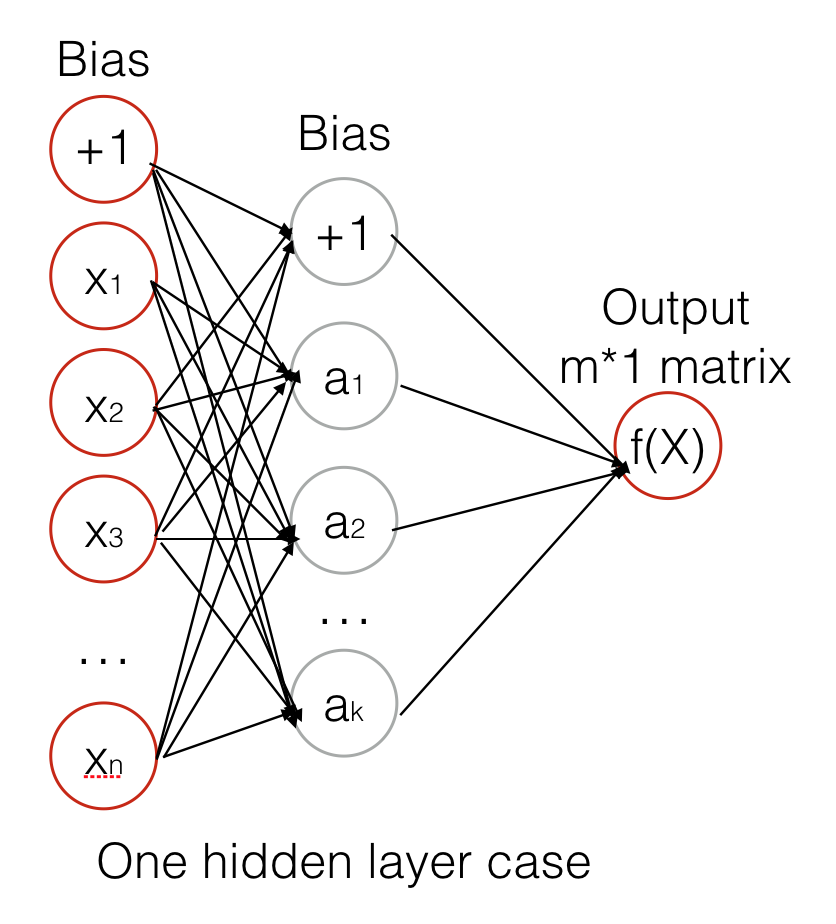
\includegraphics[scale=0.3]{2.png}
\end{center}
\paragraph{}
As someone may ask, given the logistic regression model, why do we need multilayer perceptrons to classify dataset. Comparing with logistic regression, the advantage of multilayer perceptrons is the capability to learn non-linear models. However, different random weight initializations can have different test accuracy because MLP with hidden layers have a non-convex loss function where there exists more than one local minimum. 

\subsection{Linear Support Vector Machines}
\paragraph{}
Support Vector Machine (SVM) is a supervised machine learning algorithm that builds a hyperplane in a high dimensional space which can be used in classification problems. In this algorithm, we plot each data item as a point in n-dimensional space (where n is number of features in the image) with the value of each feature being the value of a particular coordinate. Then, we perform classification by finding the hyper-plane that differentiate the two classes very well. Good separation is achieved by the hyperplane that has the largest distance to the nearest training data point of any class (functional margin).
\paragraph{}
However, in reality most of the datasets are not linearly separable. Hinge loss function can solve the problem,
\[ max(0, 1-y_i(\vec{w} \cdot \vec{x_i}-b))\]
where $y_i$ is the category for image $i$. This function is zero if $\vec{x_i}$ lies on the correct side of the margin. For data on the wrong side of the margin, the function's value is proportional to the distance from the margin. Then the optimization problem becomes to minimize\[
[\frac{1}{n}\sum_{i=1}^n max(0,1-y_i(\vec{w} \cdot \vec{x_i}-b))]+\lambda ||\vec{w} ||^2 \]
where the parameter lambda determines the tradeoff between increasing the margin-size and ensuring that $x_i$ lie on the correct size of the margin. 

\subsection{Nonlinear Support Vector Machines with Radial Basis Function Kernel}
\paragraph{}
On the base of linear support vector machine, we now introduce the kernel trick[3] that allows the algorithm to fit the maximum-margin hyperplane in a transformed feature space. Kernels are functions which takes low dimensional input space and transform it to a higher dimensional space i.e. it converts not separable problem to separable problem. There are many different kernel functions developed in the past years. Radial Basis function(RBF) kernel is one of the most popular one. The RBF kernel on two samples x and x', represented as feature vectors in some input space, is defined as
\[K(x,x') = exp(-\frac{||x-x'||^2}{2\sigma^2}) \]
\paragraph{}
Given the kernel function defined above, we take the Fourier transform of the K, and end with a Gaussian Blur function. Therefore, RBF kernel is actually a low-band pass filter [4], which is a tool to smooth image. It acts as a prior that selects out smooth solutions. Understanding how the kernel does to the data helps us to understand the performance of RBF kernel SVM. 


\section{Experiment}
\paragraph{}
In this section, we demonstrate the implementation of the above algorithms on image classification. Our task in image classification is to predict a category label for a given animal image. Images are 3-dimensional arrays of integers from 0 to 255, of size Width x Height x 3. The 3 represents the three color channels Red, Green, Blue. For the sake of our future implementation, we transferred the RGB into grayscale image.

\subsection{Data Processing}
\paragraph{}
We used some open-source software libraries to facilitate the implementation, including Scikit-learn (or ‘sklearn’) \ \url{http://scikit-learn.org/stable/}, opencv (Open Source Computer Vision Library) 
 \url{opencv.org/}, numpy \url{http://www.numpy.org/},  matplolib \url{https://matplotlib.org}, and pickle \ \url{https://docs.python.org/2/library/pickle.html}. Sklearn is a free software machine learning library for the Python. We used the logistic regression, linearSVC, rbf-kernel SVM models in sklearn, and tune the parameters based on our dataset; opencv to read and process the image data; numpy to deal with the image transformed matrix. For performance analysis, matplotlib is useful for data visualization for each model. Pickle plays an important role in saving and loading the trained model for future prediction. With these locally saved model, we created an interactive animal classification that takes in an image use would like to classify as input, the model user would like to use for prediction and returns its predicted category ID.

\subsubsection{Introduction to the COCO dataset}
\paragraph{}
COCO is a popular image recognition, segmentation, and captioning dataset with more than 30,000 images, 2 million instances, and 80 object categories. In this project, we used the 2014 dataset for detection challenge with object instance annotations provided as our primary dataset. For this dataset, there are total 82,782 images of over 90 different categories.
\paragraph{}
The dataset are in JSON format, providing comprehensive information. Each annotation instance contains a series of fields, including the category id and segmentation mask of the object, which provides information including the information of the dataset, the categories and supercategories each image belong to and information about segmentation, etc.
\paragraph{}
In this project, we looked into each annotation instance and created our final dataset using images with supercategory ‘animal.’ For this supercategory in particular, there are ten categories shown as below:
 
\begin{verbatim}
{'id': 16, 'name': 'bird', 'supercategory': 'animal'},
{'id': 17, 'name': 'cat', 'supercategory': 'animal'},
{'id': 18, 'name': 'dog', 'supercategory': 'animal'},
{'id': 19, 'name': 'horse', 'supercategory': 'animal'},
{'id': 20, 'name': 'sheep', 'supercategory': 'animal'},
{'id': 21, 'name': 'cow', 'supercategory': 'animal'},
{'id': 22, 'name': 'elephant', 'supercategory': 'animal'},
{'id': 23, 'name': 'bear', 'supercategory': 'animal'},
{'id': 24, 'name': 'zebra', 'supercategory': 'animal'},
{'id': 25, 'name': 'giraffe', 'supercategory': 'animal'}
\end{verbatim}
 
\subsubsection{Assigning training and testing data sets}
\paragraph{}
Considering the enormous size of the whole dataset, we found it infeasible to train the whole dataset based on the current device we have. Instead, we selected one supercategory 'animal', which contains ten different categories or species shown above. We first extracted all images labeled with $category\_ id$ that belongs to the supercategory 'animals,' which consist of over 19,000 images. After we obtained all animal images, we randomly sample 5,000 images as our final full dimension dataset.
\paragraph{}
We divided the dataset by assigning $3 \slash 4$ of the data, 3750 images, to our training set and the rest of $1\slash 4$, 1250 images, to the testing set. When we sampled the dataset, we shuffled the dataset so that images of most categories under this supercategory are included in the dataset.
 
\subsubsection{Data Feature and Dimension analysis}
\paragraph{}
To process the image and extract the features, we resized all images to size 256 $\times$ 256 so all entries of $X$ have the identical number of pixels. In this case, each image contains 256 $\times$ 256 features. As we discussed above that we split data in the ratio $3:1$, the dimension of training and testing set of $X$ is (3750, 256 $\times$ 256) and (1250, 256 $\times$ 256). The matrix of $X{train}$  would be in the form :
\begin{center}
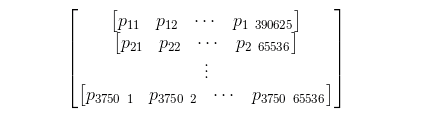
\includegraphics[scale=0.6]{6}
\end{center}
which is a column vector consists of 3,750 row vectors  where $p_{ij}$ is the $j^{th}$ pixel of the $i^{th}$ image in the dataset.
\paragraph{}
Since $Y$ for each $X$ represents the category ID, which is an integer in between 16 and 25, the dimension of training and testing set of $Y$ is (3750, 1) and  (1250, 1) respectively.
 

\subsection{Actual Implementation of Algorithms}
\paragraph{}
In terms of actual implementation, we need to tune the parameters. For multinomail logistic regression, we added a L2 regularization parameter $ \ reg=10\ $ to prevent the case of overfitting. In order to minimize the cost function, we also need to choose the slover to solve this optimization problem. With such large dataset, we tried both the default solver and the solver 'sag,' which uses a stochastic average gradient descent to compute the extremum and learn a true multinomial model. 
\paragraph{}
 For Multilayer Perceptrons neural network, our implementation used the class MLP Classifier in sklearn library. We set the solver as 'adam,' a stochastic gradient-based optimizer proposed by Kingma, Diederik, and Jimmy Ba \  \url{https://arxiv.org/abs/1412.6980}. We originally set the hidden layer size as (100,100,100), which means that the training model has three hidden layers, each contains 100 neurons. For regularization term, we also added L2 penalty  parameter.
\paragraph{}
For linear SVM algorithm, since we have 10 categories to classify, SVM need to compute the optimization 45 times (9*10/2). In Python, linear SVM is  available in scikit-learn library. We penalty parameter C of the error term as $1\slash reg$ (regularization parameter), and the loss function is default hinge loss. We use 5,000 labeled data set to train the linear SVM classifier and detail performance will be in the next section.
 

\section{Performance and Analysis}
\paragraph{}
To evaluate and compare the performance of each algorithm, we computed the training and testing accuracy of prediction of each algorithm, and we plot the confusion matrix as a tool to visualize the performance of each method.
\subsection{Evaluate Performance: Confusion Matrix}
\paragraph{}
The confusion matrix helps to visualize the performance of our classifier. To be specific, our classification system has been trained to distinguish between birds, cat, dog, horse, sheep, and cow. The confusion matrix will summarize the results of testing the algorithm for further inspection. The total number of sample is the sum of all the numbers in the cells. In this confusion matrix, of all the actual birds, 139 are predicted as birds, 24 are predicted as cat, 20 are predicted as dog, 29 are predicted as horse, 25 are predicted as sheep, 13 are predicted as cow. We can see from the matrix that the system has trouble predict cats and  dogs, but can make a pretty good prediction to birds, sheep and cow. All correct guesses are located in the diagonal of the table, so it's easy to visually inspect the table for errors, as they will be represented by values outside the diagonal. The degree of intensity of the color represents the number in each cell. As we can see, confusion matrix is a straightforward method to visualize the performance of an algorithm.

\subsection{Algorithm Performance}
\subsubsection{Logistic Regression}
When using default solver: 
\begin{enumerate}
\item Training Accuracy: 0.9880 
\item Testing Accuracy: 0.4360 
\item Time elapsed: 1815.84 seconds
\end{enumerate}
When using solver sag: 
\begin{enumerate}
\item Training Accuracy: 0.9899
\item Testing Accuracy: 0.4200
\item Time elapsed: 2172.96 seconds
\end{enumerate}

Confusion matrix analysis: \\
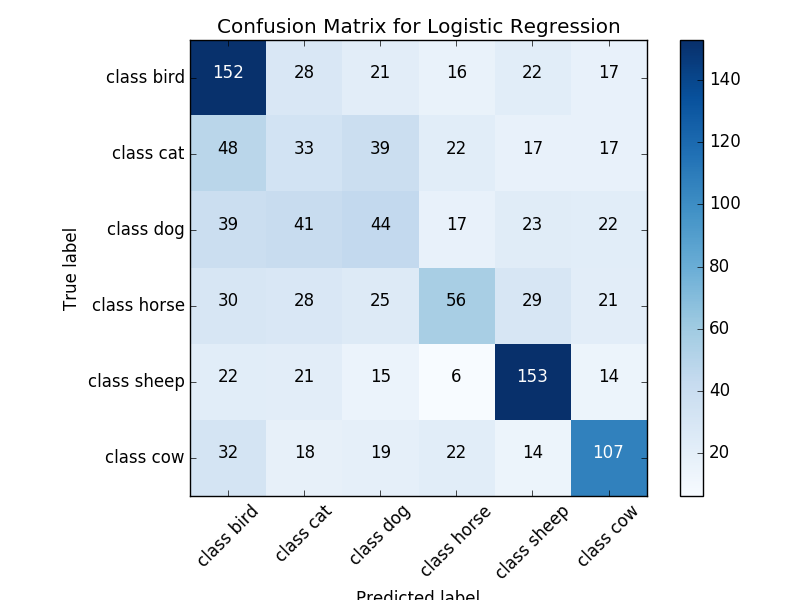
\includegraphics[scale=0.4]{logreg_cm_new.png}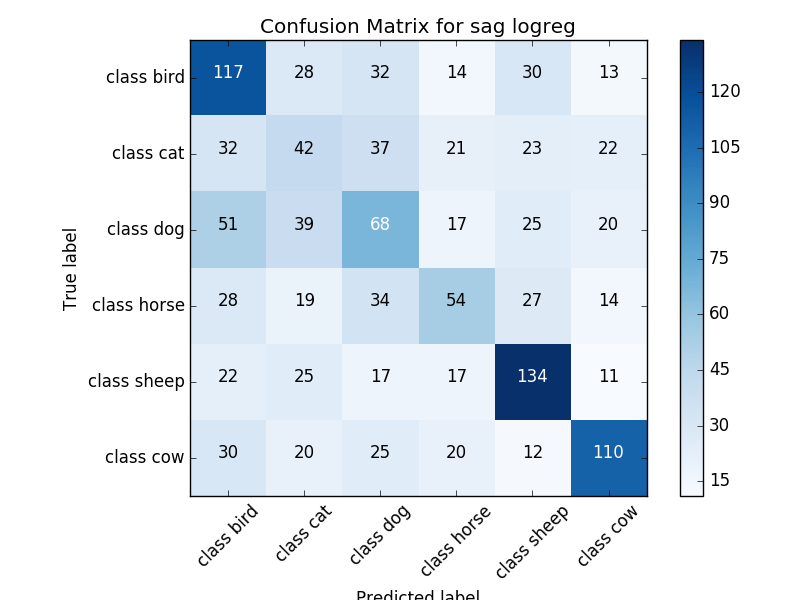
\includegraphics[scale=0.4]{sag_cm_new.png}

\subsection{Performance of Multilayer Perceptrons}
(Before) Parameters: Hidden layer (100,100,100) 
\begin{enumerate}
\item Training accuracy: 0.1971
\item Training accuracy: 0.1971
\item Time elapsed: 121.34 seconds 
\end{enumerate}
(After) Parameters: Hidden layer (500,500,500).\\ We downsized all images to 25$ \times $ 25 and increased the number of neurons of each layer. 
\begin{enumerate}
\item Training accuracy: 0.9669
\item Testing accuracy: 0.4488
\item Time elapsed: 55.79 seconds
\end{enumerate}
Confusion matrix analysis: \\
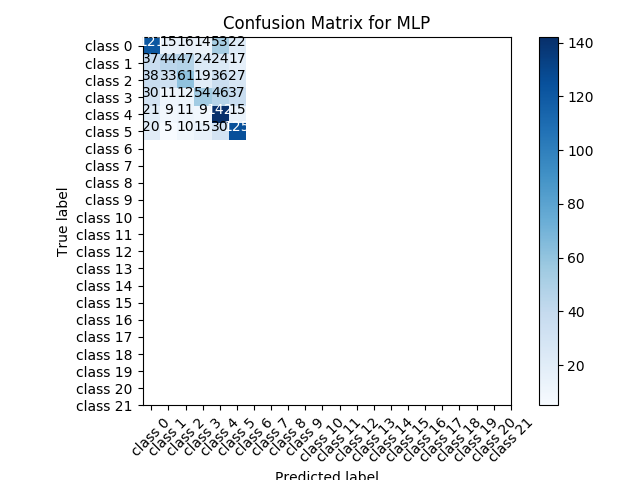
\includegraphics[scale=0.4]{MLP_cm.png}
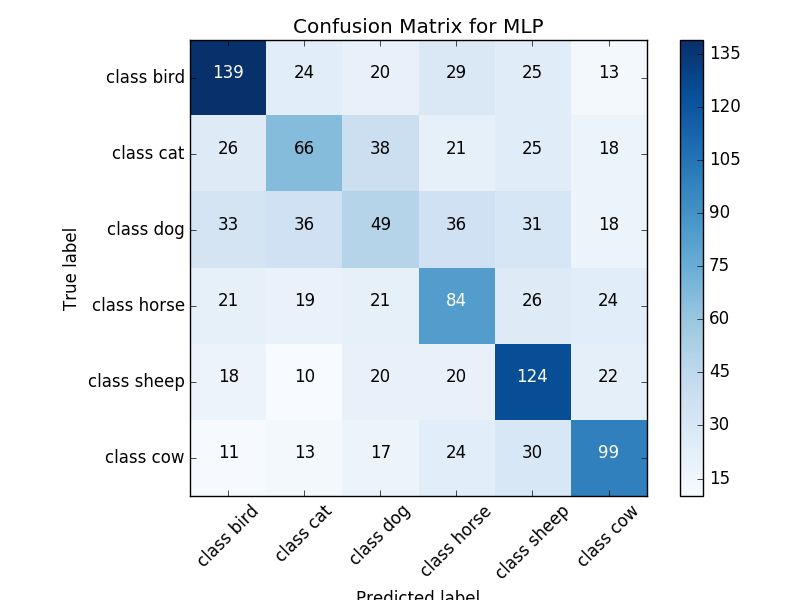
\includegraphics[scale=0.4]{MLP_cm_new1.png}

\subsection{Performance of Linear SVM}
\begin{enumerate}
\item Training Accuracy: 0.9896
\item Testing Accuracy: 0.4240
\item Time elapsed: 3691.60 seconds
\end{enumerate}
Confusion matrix analysis: 
\begin{center}
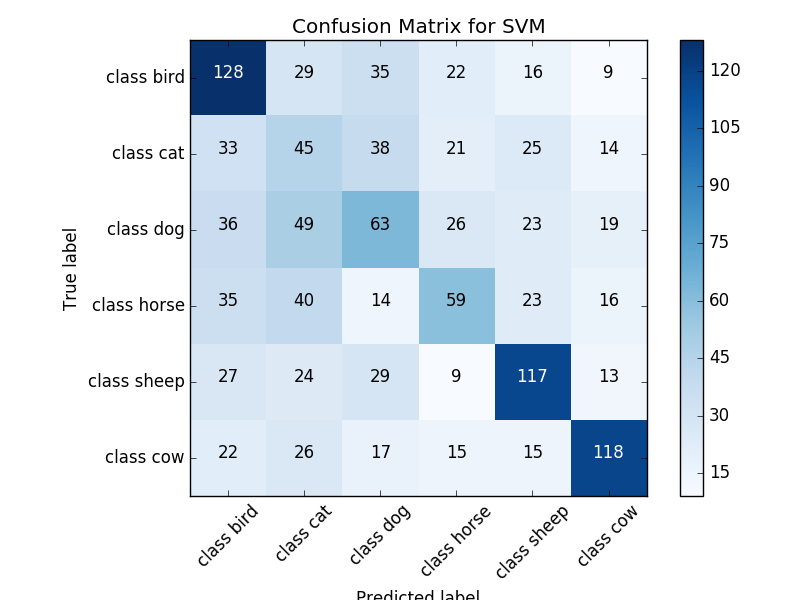
\includegraphics[scale=0.4]{svm_cm_new.png}
\end{center}

\subsection{Performance of Kernel SVM}
\begin{enumerate}
\item Training Accuracy: 0.9909
\item Testing Accuracy: 0.4704
\item Time elapsed: 1522.64 seconds
\end{enumerate}
Confusion matrix analysis: \begin{center}
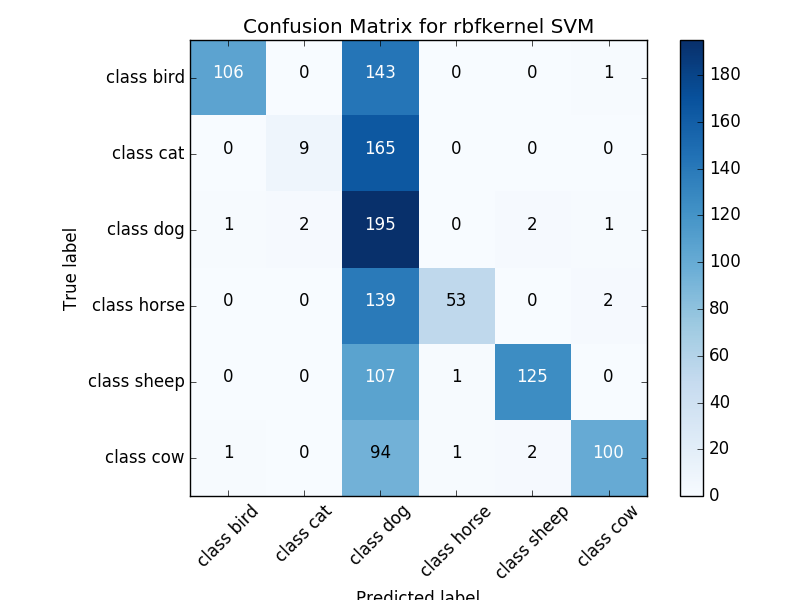
\includegraphics[scale=0.4]{kernelSVM_cm_new.png}
\end{center}
\section{Conclusion}
Run time:  MLP > Logistic Regression > Linear SVM
Testing Accuracy: MLP > Logistic Regression > Linear SVM
Wow! Neural Network is the best!

\section{Future Work}
We are gonna run GPU to train larger dataset.
Use Kernel SVM as classifier.
Tune the parameters!
Regularization parameter
Number of layers and neurons
Different random weight initializations 

\section*{Acknowledgement}
We would like to thank Prof.Gu and our grutors Maggie and Zhepei for their help throughout this course.

\section*{References}
\small
[1] Vapnik,\ V., Golowich,\ S.\ E., \& Smola,\ A.\ J. (1997). Support vector method for function approximation, regression estimation and signal processing. In Advances in neural information processing systems (pp. 281-287).
[2] Chang, Y.\ W., Hsieh, C.\ J., Chang, K.\ W., Ringgaard, M., \& Lin, C.\ J. (2010). Training and testing low-degree polynomial data mappings via linear SVM. Journal of Machine Learning Research, 11(Apr), 1471-1490.
\end{document}